% --------------------------- Implementation ---------------------------------


\section{Implementation}

\begin{figure}[h!]  
    \centering
    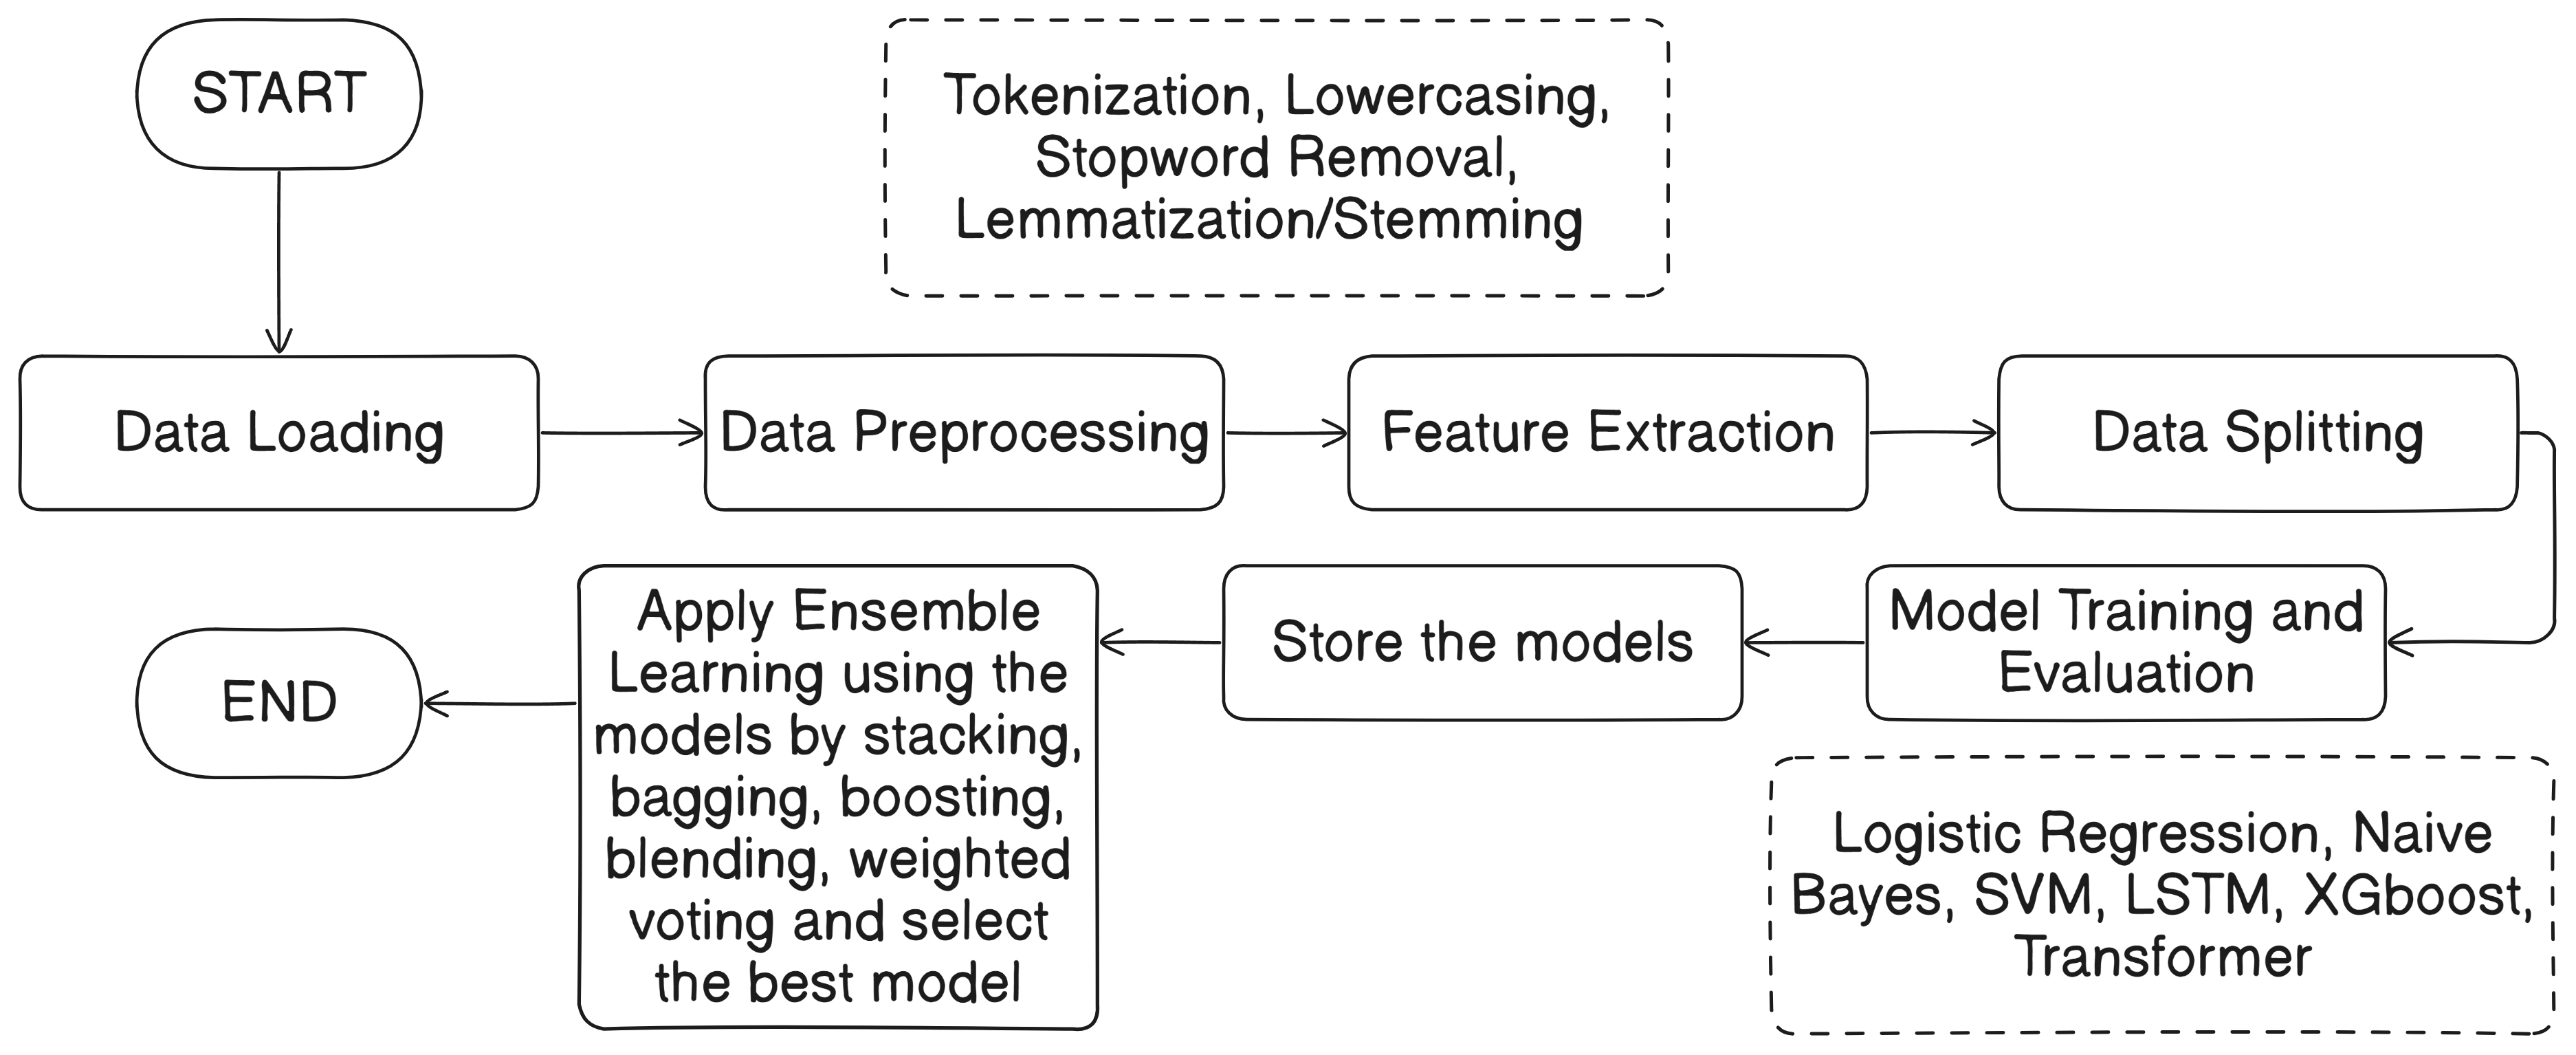
\includegraphics[width=1.0\textwidth]{Images/ML Model Workflow.png}  
    \caption{Workflow for getting the model for the web application}
    \label{model workflow}  % Label for referencing the figure
\end{figure}


\subsection{Data Collection and Dataset Preparation}
\begin{table}[H]
    \centering
    \caption*{Stepwise Algorithm for Data Collection and Dataset Combination}
    \label{tab:algorithm}
    \setlength{\arrayrulewidth}{1pt}
    \begin{tabularx}{\textwidth}{|c|X|}
        \hlineB{1.0}
        \rowcolor{lightestgray}
        \textbf{Step} & \textbf{Description} \\
        \hlineB{1.0}
        1 & \textbf{Import Libraries:} Import \texttt{praw, pandas, time} for data collection and \texttt{sklearn.utils.shuffle} for combining datasets. \\
        \hlineB{1.0}
        2 & \textbf{Initialize Reddit API:} Use the provided credentials (\texttt{client\_id}, \texttt{client\_secret}, \texttt{user\_agent}) to create a Reddit instance. \\
        \hlineB{1.0}
        3 & \textbf{Define Subreddits and Labels:} Create a dictionary mapping labels to subreddit lists:
            \begin{itemize}[noitemsep, topsep=0pt]
                \item \textbf{normal}: \texttt{news, AskReddit}
                \item \textbf{depression}: \texttt{depression}
                \item \textbf{ptsd}: \texttt{PTSD}
                \item \textbf{anxiety}: \texttt{Anxiety}
                \item \textbf{bipolar}: \texttt{BipolarReddit}
            \end{itemize} \\
        \hlineB{1.0}
        4 & \textbf{Set Post Types and Limit:} Define post types (\texttt{hot, new, top}) and set \texttt{posts\_per\_type} to 100. \\
        \hlineB{1.0}
        5 & \textbf{Collect Posts:}
            \begin{itemize}[noitemsep, topsep=0pt]
                \item For each label and its associated subreddits, iterate over each post type.
                \item Retrieve posts from the subreddit (using the corresponding post type and a limit of 100).
                \item For each post, combine the title and selftext, and append the result along with its label to a data list.
                \item Pause for 1 second between requests.
            \end{itemize} \\
        \hlineB{1.0}
    \end{tabularx}
\end{table}

\begin{table}[H]
    \centering
    \caption*{Stepwise Algorithm for Data Collection and Dataset Combination}
    \label{tab:algorithm}
    \setlength{\arrayrulewidth}{1pt}
    \begin{tabularx}{\textwidth}{|c|X|}
        \hlineB{1.0}
        \rowcolor{lightestgray}
        \textbf{Step} & \textbf{Description} \\
        \hlineB{1.0}
        6 & \textbf{Save Collected Data:} Convert the data list into a DataFrame with columns \texttt{text} and \texttt{label} and save it as \texttt{\{label\}\_dataset.csv}. \\
        \hlineB{1.0}
        7 & \textbf{Load Datasets:} Read the individual CSV files for \texttt{bipolar, depression, normal, anxiety,} and \texttt{ptsd} into separate DataFrames. \\
        \hlineB{1.0}
        8 & \textbf{Determine Minimum Length:} Compute \texttt{min\_length} as the minimum number of records among datasets (using \texttt{len(normal\_df)//6} for the normal dataset to balance its count). \\
        \hlineB{1.0}
        9 & \textbf{Create a Balanced Pattern:}
            \begin{itemize}[noitemsep, topsep=0pt]
                \item Loop from 0 to \texttt{min\_length - 1}.
                \item For each iteration, append to a new list:
                    \begin{itemize}[noitemsep, topsep=0pt]
                        \item The \texttt{i\textsuperscript{th}} record from \texttt{bipolar\_df}.
                        \item The \texttt{i\textsuperscript{th}} record from \texttt{depression\_df}.
                        \item Six consecutive records from \texttt{normal\_df} (indices \texttt{i*6} to \texttt{(i+1)*6}).
                        \item The \texttt{i\textsuperscript{th}} record from \texttt{anxiety\_df}.
                        \item The \texttt{i\textsuperscript{th}} record from \texttt{ptsd\_df}.
                    \end{itemize}
            \end{itemize} \\
        \hlineB{1.0}
        10 & \textbf{Convert to DataFrame:} Transform the balanced list into a DataFrame (\texttt{pattern\_df}). \\
        \hlineB{1.0}
        11 & \textbf{Prepare Remaining Data:} Concatenate the leftover records from each dataset (beyond \texttt{min\_length} for all datasets and beyond \texttt{min\_length*6} for the normal dataset) and shuffle them. \\
        \hlineB{1.0}
        12 & \textbf{Merge and Save Final Dataset:} Combine \texttt{pattern\_df} with the shuffled remaining data, reset the index, and save the final DataFrame as \texttt{mental\_health\_combined.csv}. \\
        \hlineB{1.0}
    \end{tabularx}
\end{table}

\begin{figure}[h!]  
    \centering
    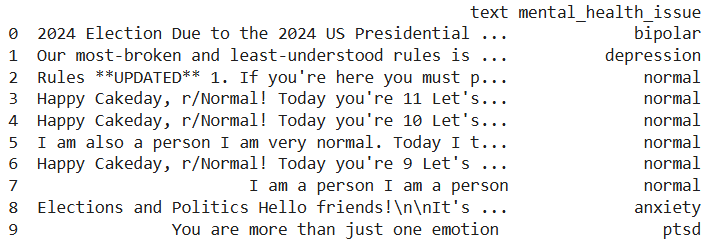
\includegraphics[width=0.9\textwidth]{Images/Dataset.png}  
    \caption{Obtained Dataset}
    \label{LSTMROC711}  % Label for referencing the figure
\end{figure}


% ----- adding subreddit info ------

\begin{figure}[h!]  
    \centering
    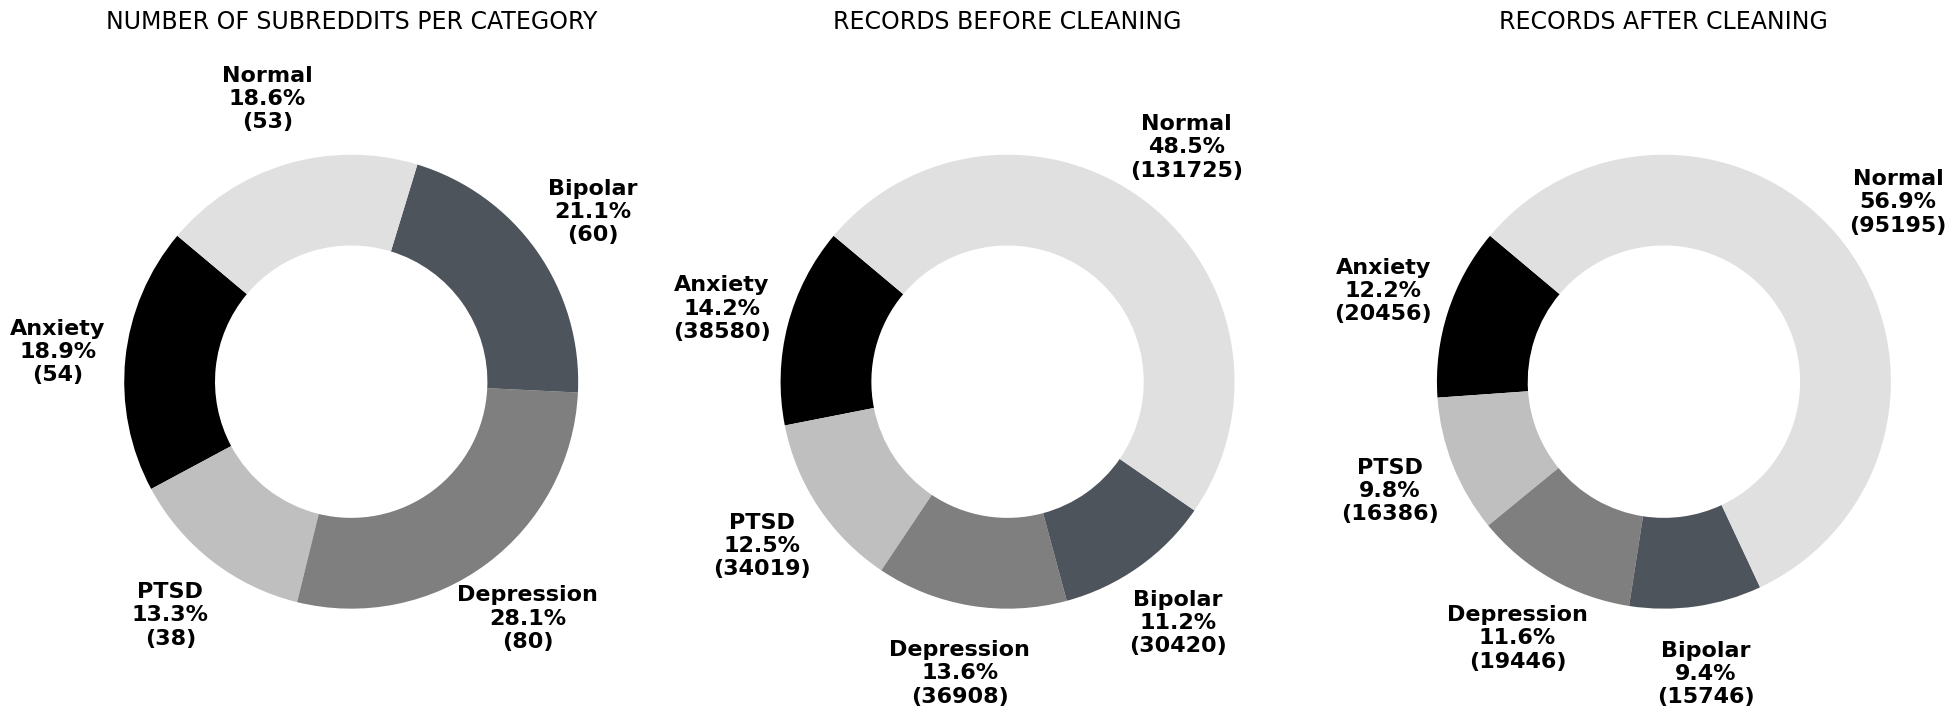
\includegraphics[width=1.0\textwidth]{Images/Data Collection Graph.png}  
    \caption{Collected Data Statistics}
    \label{LSTMROC7uyiut11}  % Label for referencing the figure
\end{figure}

\noindent
The dataset for mental health classification was compiled from subreddit communities, initially containing 385,800 records across five categories: anxiety (54 subreddits), PTSD (38), depression (80), bipolar disorder (60), and normal mental states (53). After data cleaning to ensure quality and relevance, the dataset was reduced to 167,279 records. A subset of 18,596 cleaned records was used for analysis to address computational constraints, such as memory and processing power, which would make training on the full dataset infeasible on standard hardware. This approach balances efficiency and performance, enabling faster experimentation and iterative model improvement while maintaining a representative sample.


% ----------------- Data Preprocessing



\subsection{Data Cleaning and Feature Extraction}

\begin{table}[H]
    \caption*{Stepwise Algorithm for Data Cleaning and Feature Extraction}
    \label{tab:algorithm}
    \setlength{\arrayrulewidth}{1pt}
    \centering
    \begin{tabularx}{\textwidth}{|c|X|}
    \hlineB{1.0}
    \rowcolor{lightestgray}
    \textbf{Step} & \textbf{Description} \\
    \hlineB{1.0}
    1 & \textbf{Import Libraries \& Resources}: Import \texttt{pandas}, \texttt{re}, \texttt{TfidfVectorizer} from scikit-learn, and NLTK modules. Download the necessary NLTK resources (e.g., \texttt{stopwords}, \texttt{punkt}, and \texttt{punkt\_tab}). \\
    \hlineB{1.0}
    2 & \textbf{Load Dataset}: Read the CSV file \texttt{mental\_health.csv} into a pandas DataFrame. \\
    \hlineB{1.0}
    3 & \textbf{Handle Missing Values}: Drop any rows where the \texttt{text} field is missing. \\
    \hlineB{1.0}
    4 & \textbf{Remove Duplicates}: Eliminate duplicate rows based on the \texttt{text} column. \\
    \hlineB{1.0}
    5 & \textbf{Define Negative Words}: Create a set of negative words (e.g., \texttt{not}, \texttt{no}, \texttt{nor}, etc.) that will be retained during stopword removal. \\
    \hlineB{1.0}
    6 & \textbf{Define Cleaning Function}: Write the function \texttt{clean\_text(text)} to preprocess text by:
        
      \begin{enumerate}[label=(\alph*), itemsep=0pt, topsep=0pt, partopsep=0pt, parsep=0pt]
        \item Removing URLs using regex.
        \item Removing mentions (e.g., \texttt{@username}).
        \item Removing special characters, numbers, and punctuation.
        \item Converting text to lowercase.
        \item Tokenizing the text using NLTK's \texttt{word\_tokenize}.
        \item Removing stopwords (while keeping negative words).
        \item Rejoining tokens into a cleaned string.
      \end{enumerate} \\
    \hlineB{1.0}
\end{tabularx}
\end{table}

\begin{table}[H]
    \caption*{Stepwise Algorithm for Data Cleaning and Feature Extraction}
    \label{tab:algorithm}
    \setlength{\arrayrulewidth}{1pt}
    \centering
    \begin{tabularx}{\textwidth}{|c|X|}
    \hlineB{1.0}
    \rowcolor{lightestgray}
    \textbf{Step} & \textbf{Description} \\
    \hlineB{1.0}
    7 & \textbf{Apply Cleaning Function}: Execute \texttt{clean\_text} on the \texttt{text} column and store the result in a new column called \texttt{cleaned\_text}. \\
    \hlineB{1.0}
    8 & \textbf{Initialize TF-IDF Vectorizer}: Create a TF-IDF vectorizer instance with a maximum of 10,000 features. (Other methods include Bag-Of-Words, LIWC, N-Gram, Word2Vec)\\
    \hlineB{1.0}
    9 & \textbf{Fit \& Transform Data}: Apply the vectorizer to the \texttt{cleaned\_text} to generate the TF-IDF feature matrix \texttt{X}. \\
    \hlineB{1.0}
    10 & \textbf{Optional - Convert to DataFrame}: Convert the TF-IDF sparse matrix \texttt{X} into a pandas DataFrame for easier inspection (e.g., print the first few rows). \\
    \hlineB{1.0}
    11 & \textbf{Optional - Save Preprocessed Data}: Save the final preprocessed DataFrame to \texttt{preprocessed\_mental\_health.csv}. \\
    \hlineB{1.0}
    \end{tabularx}
\end{table}

\begin{figure}[h!]  
    \centering
    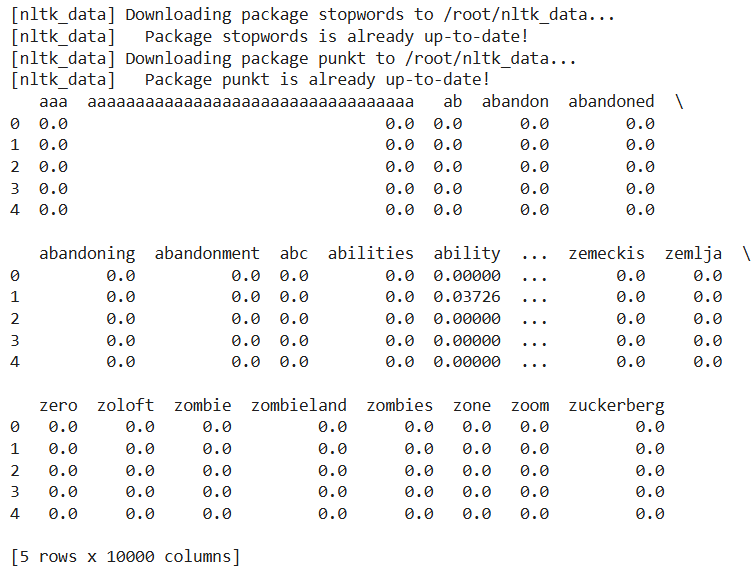
\includegraphics[width=0.9\textwidth]{Images/Data Cleaning and Preprocessing.png}  
    \caption{Output of TF-IDF Vectorization}
    \label{Data Collection and Preprocessing}  % Label for referencing the figure
\end{figure}

\noindent \textbf{Datasets:} \\
\textbf{Before Cleaning:} \texttt{mental\_health.csv} \\
\textbf{After Cleaning:} \texttt{preprocessed\_mental\_helth.csv}

\vspace{1em} % Adds a small vertical space

\begin{table}[H]
    \centering
    \setlength{\arrayrulewidth}{1pt}
    \begin{tabularx}{\textwidth}{|c|X|X|}
    \hlineB{1.0}
    \rowcolor{lightestgray}
    \textbf{Stage} & \textbf{Schema} & \textbf{Description} \\
    \hlineB{1.0}
    \makecell{Before\\Cleaning} &
    \begin{tabular}[t]{@{}l@{}}
    \texttt{text}: Original text data \\
    \texttt{mental\_issue}: Mental health \\ \quad \quad \quad \quad \quad \quad \quad \ \ issues
    \end{tabular}
    &
    Contains raw, unprocessed text data with possible missing values, duplicates, URLs, mentions, and special characters. \\[6pt]
    \hlineB{1.0}
    \makecell{After\\Cleaning} &
    \begin{tabular}[t]{@{}l@{}}
    \texttt{text}: Original text data \\
    \texttt{mental\_issue}: Mental health \\ \quad \quad \quad \quad \quad \quad \quad \ \ issues \\
    \texttt{cleaned\_text}: Processed text \\ \quad \quad \quad \quad \quad \quad \quad \ \ data
    \end{tabular}
    &
    Data is cleaned by removing URLs, mentions, special characters, and extra noise. The text is converted to lowercase, tokenized, stopwords (except key negative words) are removed, and the cleaned text is stored in the new column \texttt{cleaned\_text}. \\[6pt]
    \hlineB{1.0}
    \end{tabularx}
    \caption*{Dataset Schema Before and After Data Cleaning}
    \label{tab:dataset_schema}
\end{table}

\noindent
The matrix dimensions for Bag of Words are determined by the number of records, which is 18,597 in this case, and the size of the vocabulary, which represents the number of unique words in the \texttt{cleaned\_text} column. Similarly, for TF-IDF, the dimensions of the matrix are the same as BOW, calculated as the number of records multiplied by the vocabulary size. For N-gram, the matrix size depends on the range of n-grams used. For example, a unigram produces dimensions equivalent to BOW, while bigram or trigram models increase the vocabulary size due to the inclusion of word combinations. Word2Vec, on the other hand, creates a dense vector representation for each word, with dimensions based on the predefined vector size, such as 100 or 200. Aggregating these vectors at the sentence level, typically by averaging, results in a matrix of dimensions equal to the number of records multiplied by the vector dimensions. For LIWC, the dimensions are determined by the number of predefined LIWC categories, which is typically around 70. The resulting matrix dimensions are the number of records multiplied by the number of LIWC categories.

% -------- logistic regression

\subsection{Machine Learning Models}

Algorithms like Logistic Regression, K-Nearest Neighbors, Support Vector Machine, Random Forest, XGBoost and Naive Bayes are implemented for the classification of mental health issues. The code algorithm below demonstrates the implementation. The models are evaluated on the test set using metrics like accuracy and classification reports. Hyperparameter Tuning is performed using RandomizedSearchCV to optimize the model performance. Naive Bayes model after hyperparamter tuning is selected along with the basic Logistic Regression, Support Vector Machine, XGboost for the final ensemble model for the web application. 

\begin{table}[H]
    \caption*{\textbf{Stepwise Algorithm for Machine Learning Models}}
    \label{tab:stepwise_algorithm}
    \centering
    \renewcommand{\arraystretch}{1.2}
    \small
    \setlength{\arrayrulewidth}{1pt}
    \begin{tabularx}{\textwidth}{|c|X|}
        \hlineB{1.0}
        \rowcolor{lightestgray}
        \textbf{Step} & \textbf{Description} \\
        \hlineB{1.0}
        1 & \textbf{Data Loading and Verification:} Load the dataset (\texttt{preprocessed\_mental\_health.csv}) using pandas, verify required columns (\texttt{cleaned\_text} and \texttt{mental\_health\_issue}), and drop rows with missing values. \\
        \hlineB{1.0}
        2 & \textbf{Tokenization and Feature Extraction:} Choose a method (Bag-of-Words, TF-IDF, LIWC, Word2Vec, or N-gram) and transform \texttt{cleaned\_text} into a numerical feature matrix $X$. \\
        \hlineB{1.0}
        3 & \textbf{Target Variable Preparation:} Extract the target variable $y$ from the \texttt{mental\_health\_issue} column. \\
        \hlineB{1.0}
        4 & \textbf{Dataset Splitting:} Split $X$ and $y$ into training and test sets (e.g., 80/20 split) using \texttt{train\_test\_split} with a fixed random state. \\
        \hlineB{1.0}
        5 & \textbf{Model Initialization:} For each algorithm (Logistic Regression, Naive Bayes, SVM, KNN, Random Forest, XGBoost), initialize the model with appropriate hyperparameters. \\
        \hlineB{1.0}
        6 & \textbf{Model Training:} Train the selected model on the training data. \\
        \hlineB{1.0}
        7 & \textbf{Prediction:} Use the trained model to predict mental health issues on the test set. \\
        \hlineB{1.0}
        8 & \textbf{Model Evaluation:} Evaluate performance by computing accuracy, classification reports, and confusion matrices. \\
        \hlineB{1.0}
        9 & \textbf{Cross-Validation:} Apply Stratified K-Fold (e.g., 5 folds) cross-validation to record accuracies and calculate the mean and standard deviation. \\
        \hlineB{1.0}
        10 & \textbf{Performance Comparison:} Compare evaluation metrics across all models and feature extraction methods to select the best combination. \\
        \hlineB{1.0}
        11 & \textbf{Hyperparameter Tuning:} For Logistic Regression, Naive Bayes, SVM, and KNN, optimize hyperparameters using \texttt{RandomizedSearchCV} to search the parameter space and select the optimal configuration. \\
        \hlineB{1.0}
    \end{tabularx}
\end{table}



\subsection{Deep Learning Models}

\begin{table}[H]
    \caption*{\textbf{Stepwise Algorithm for LSTM-based Model}}
    \label{tab:lstm_algorithm}
    \centering
    \renewcommand{\arraystretch}{1.3}
    \small
    \setlength{\arrayrulewidth}{1pt}
    \begin{tabularx}{\textwidth}{|c|X|}
        \hlineB{1.0}
        \rowcolor{lightestgray}
        \textbf{Step} & \textbf{Description} \\
        \hlineB{1.0}
        1 & \textbf{Data Loading:} Load \texttt{preprocessed\_mental\_health.csv} using pandas. \\
        \hlineB{1.0}
        2 & \textbf{Feature \& Target Preparation:}  
              \begin{itemize}[noitemsep, topsep=0pt]
                  \item Extract text ($X$) and target ($y$).
                  \item Encode $y$ using \texttt{LabelEncoder} and convert to one-hot with \texttt{to\_categorical}.
              \end{itemize} \\
        \hlineB{1.0}
        3 & \textbf{Tokenization \& Padding:}  
              \begin{itemize}[noitemsep, topsep=0pt]
                  \item Initialize Keras \texttt{Tokenizer} with \texttt{num\_words=25000}.
                  \item Fit on $X$, convert texts to sequences, and pad to \texttt{max\_length=128} using \texttt{pad\_sequences}.
              \end{itemize} \\
        \hlineB{1.0}
        4 & \textbf{Cross-Validation Setup:} Define a 5-fold StratifiedKFold (shuffle=True, random\_state=42). \\
        \hlineB{1.0}
    \end{tabularx}
\end{table}

\begin{table}[H]
    \caption*{\textbf{Stepwise Algorithm for LSTM-based Model}}
    \label{tab:lstm_algorithm}
    \centering
    \renewcommand{\arraystretch}{1.3}
    \small
    \setlength{\arrayrulewidth}{1pt}
    \begin{tabularx}{\textwidth}{|c|X|}
        \hlineB{1.0}
        \rowcolor{lightestgray}
        \textbf{Step} & \textbf{Description} \\
        \hlineB{1.0}
        5 & \textbf{LSTM Model Building:} For each fold, build a Keras Sequential model with:
              \begin{itemize}[noitemsep, topsep=0pt]
                  \item \texttt{Embedding(vocab\_size, 128, input\_length=128)}
                  \item \texttt{LSTM(128, return\_sequences=True)}
                  \item \texttt{Dropout(0.2)}
                  \item \texttt{LSTM(64)}
                  \item \texttt{Dropout(0.2)}
                  \item \texttt{Dense(64, activation='relu')}
                  \item \texttt{Dense(num\_classes, activation='softmax')}
              \end{itemize} \\
        \hlineB{1.0}
        6 & \textbf{Model Training:} Compile the model with \texttt{optimizer='adamw'} and \texttt{loss='categorical\_crossentropy'}. Train for 20 epochs with a batch size of 16 using the training fold and validate on the validation fold. \\
        \hlineB{1.0}
        7 & \textbf{Evaluation per Fold:} 
              \begin{itemize}[noitemsep, topsep=0pt]
                  \item Evaluate the model on the validation set to obtain loss and accuracy.
                  \item Predict probabilities on the validation set and compute the confusion matrix.
              \end{itemize} \\
        \hlineB{1.0}
        8 & \textbf{ROC Curve Calculation:}  
              \begin{itemize}[noitemsep, topsep=0pt]
                  \item Concatenate true labels and predictions from all folds.
                  \item Binarize true labels and compute ROC curves and AUC for each class plus a micro-average.
              \end{itemize} \\
        \hlineB{1.0}
        9 & \textbf{Visualization:} Plot ROC curves, validation loss/accuracy across folds, and the average confusion matrix using Matplotlib and Seaborn. \\
        \hlineB{1.0}
        10 & \textbf{Final Evaluation:} Compute the average cross-validated accuracy and display a classification report. \\
        \hlineB{1.0}
    \end{tabularx}
\end{table}


\begin{figure}[h!]  
    \centering
    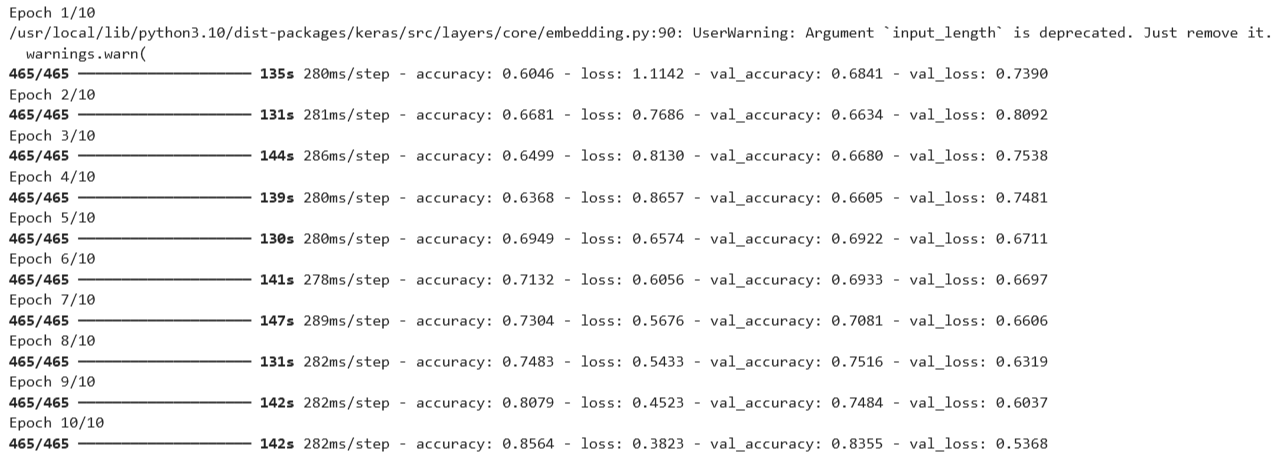
\includegraphics[width=1.0\textwidth]{Images/LSTM Epoch.png}  
    \caption{Output for LSTM Epochs}
    \label{LSTm Epochs}  % Label for referencing the figure
\end{figure}

\pagebreak

\begin{figure}[h!]  
    \centering
    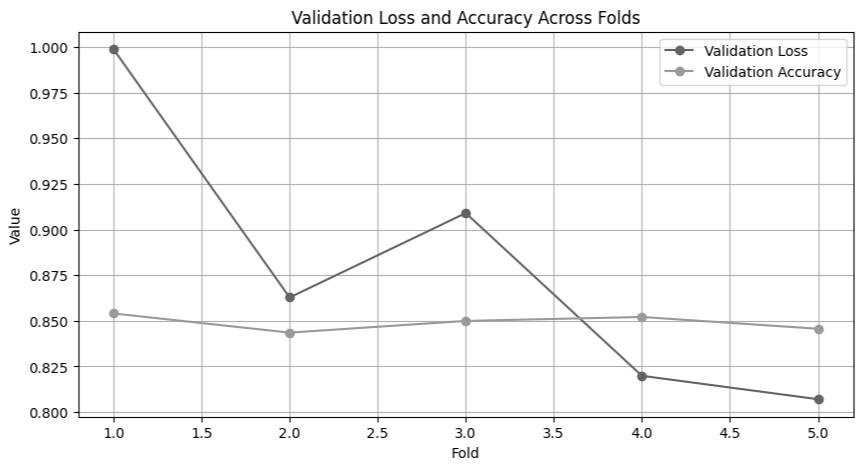
\includegraphics[width=1.0\textwidth]{Images/LSTM LA.png}  
    \caption{LSTM Validation loss and accuracy}
    \label{Accuracy Loss}  % Label for referencing the figure
\end{figure}

\begin{figure}[h!]  
    \centering
    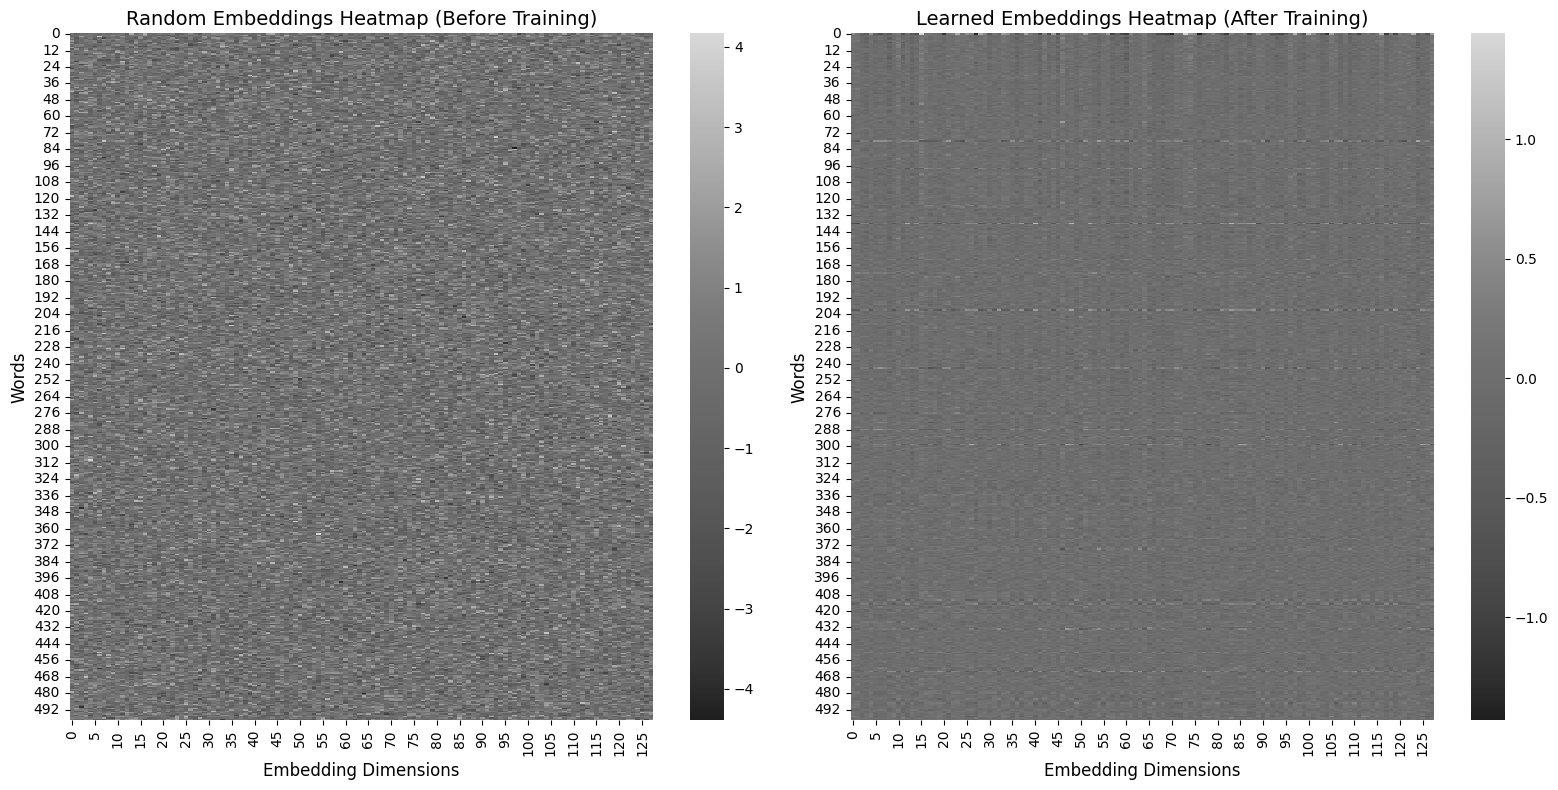
\includegraphics[width=1.0\textwidth]{Images/LSTM EMBED.png}  
    \caption{LSTM Random and Learned Embeddings}
    \label{lstm embed}  % Label for referencing the figure
\end{figure}

\pagebreak

\begin{figure}[h!]  
    \centering
    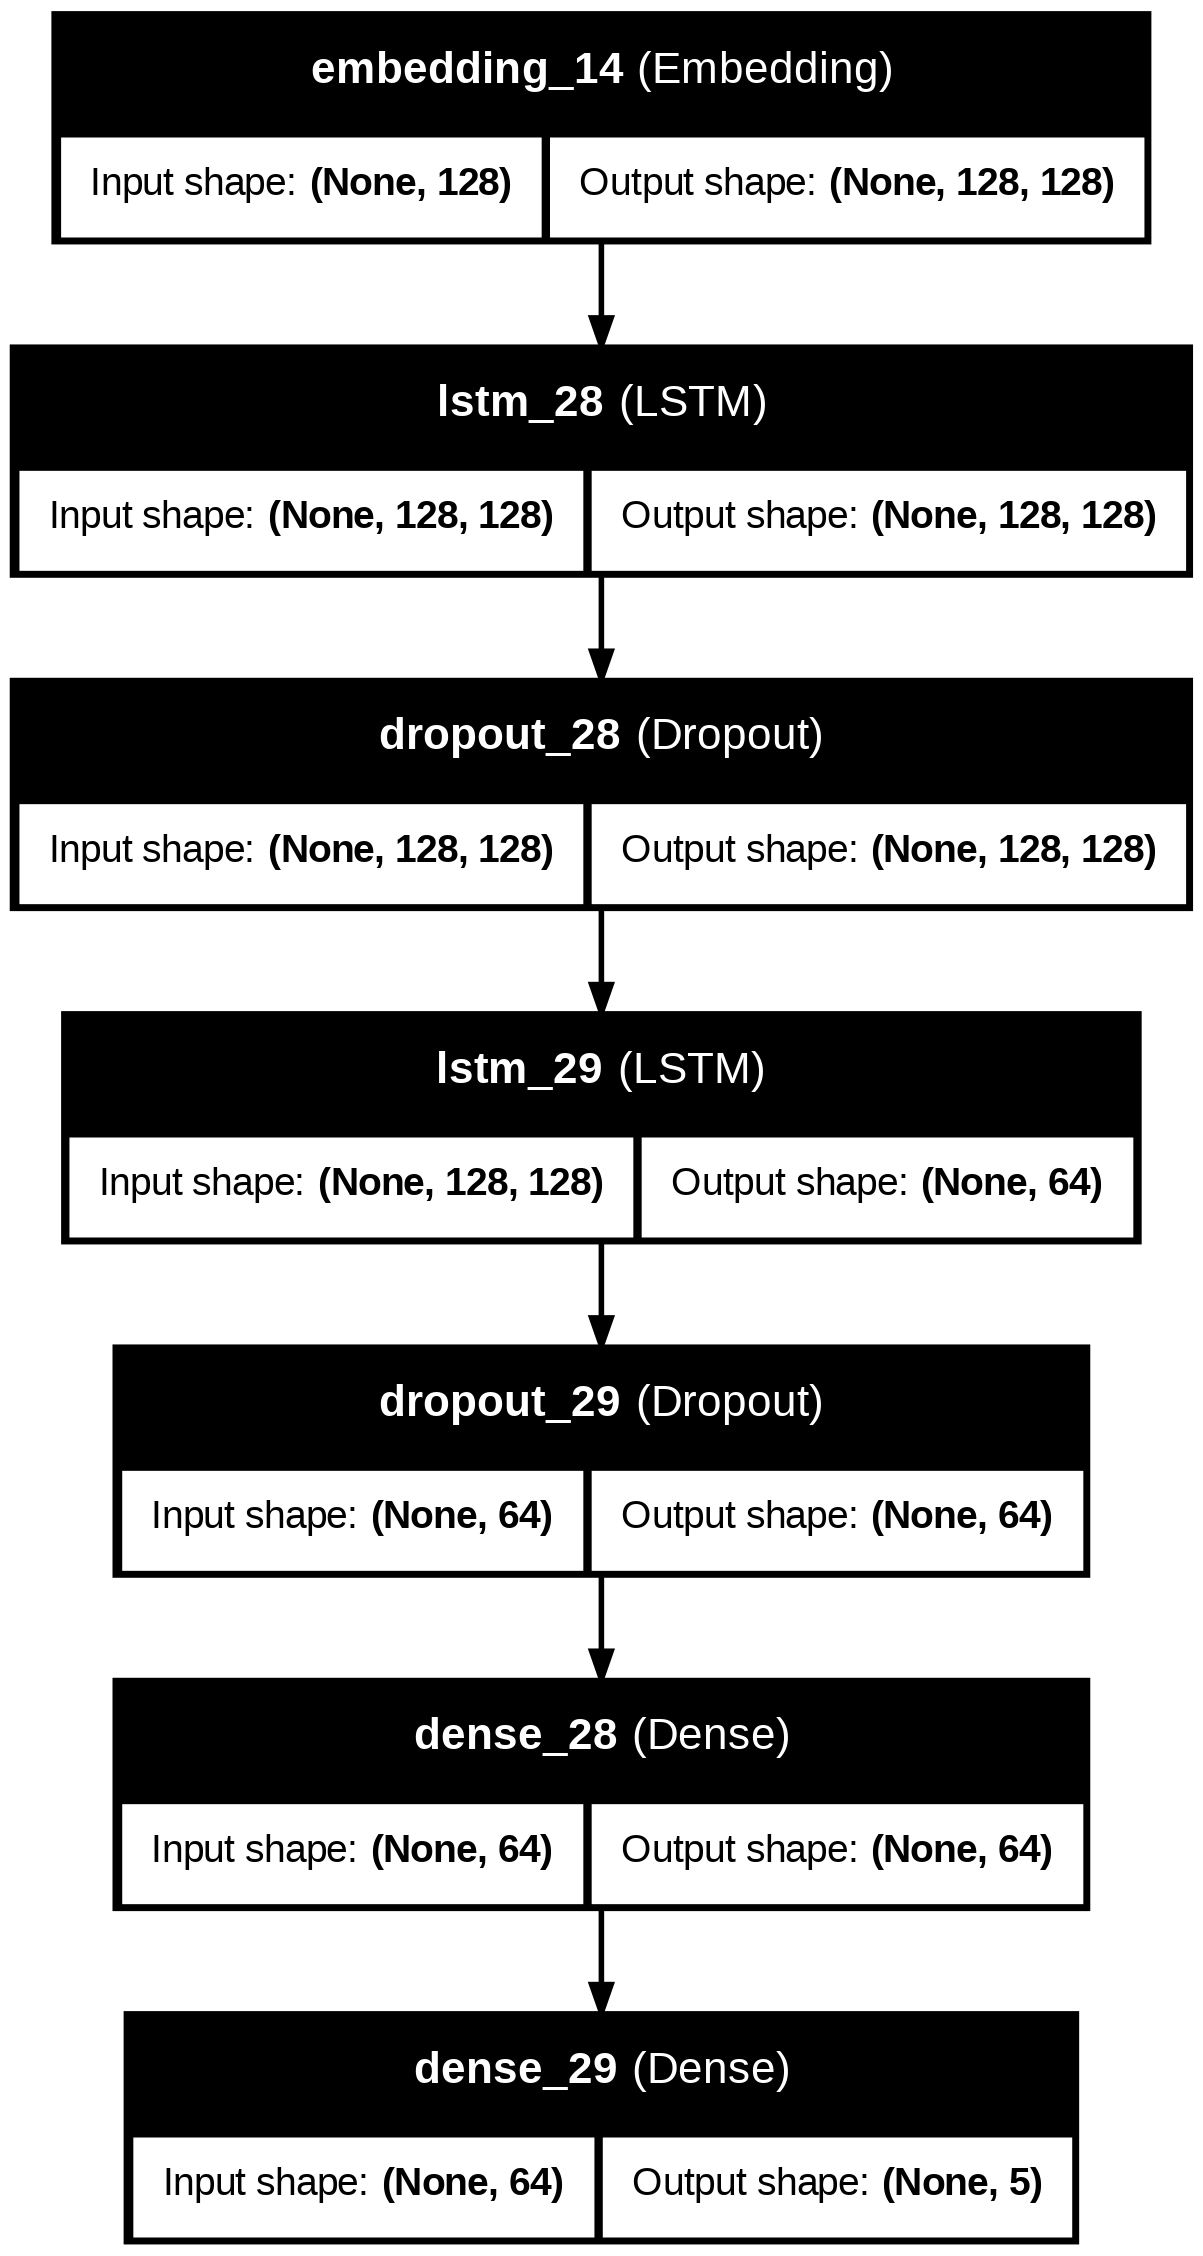
\includegraphics[width=0.45\textwidth]{Images/LSTM MODEL.png}  
    \caption{LSTM Model Architecture}
    \label{lstm arch}  % Label for referencing the figure
\end{figure}


\begin{table}[H]
    \caption*{\textbf{Stepwise Algorithm for Custom Transformer-based Model}}
    \label{tab:transformer_algorithm}
    \centering
    \renewcommand{\arraystretch}{1.3}
    \small
    \setlength{\arrayrulewidth}{1pt}
    \begin{tabularx}{\textwidth}{|c|X|}
        \hlineB{1.0}
        \rowcolor{lightestgray}
        \textbf{Step} & \textbf{Description} \\
        \hlineB{1.0}
        1 & \textbf{Import Libraries:} Import required packages including NumPy, pandas, Matplotlib, Seaborn, scikit-learn modules (e.g., \texttt{LabelEncoder}, \texttt{confusion\_matrix}), and TensorFlow Keras modules (e.g., \texttt{TextVectorization}, \texttt{Embedding}, \texttt{LSTM}, \texttt{MultiHeadAttention}, etc.). \\
        \hlineB{1.0}
        2 & \textbf{Load Dataset:} Use Google Colab's file upload to import \texttt{preprocessed\_mental\_health.csv}. Drop rows with missing \texttt{cleaned\_text} and extract features (\texttt{texts}) and labels (\texttt{labels}). \\
        \hlineB{1.0}
        3 & \textbf{Preprocess Labels:} Encode labels with \texttt{LabelEncoder}, convert them to one-hot format via \texttt{to\_categorical}, and retrieve class names. \\
        \hlineB{1.0}
        4 & \textbf{Text Vectorization:} Set \texttt{vocab\_size = 25000} and \texttt{sequence\_length = 300}. Create a \texttt{TextVectorization} layer, adapt it on the input texts (using a TensorFlow \texttt{Dataset}), and vectorize the texts. \\
        \hlineB{1.0}
    \end{tabularx}
\end{table}

\begin{table}[H]
    \caption*{\textbf{Stepwise Algorithm for Custom Transformer-based Model}}
    \label{tab:transformer_algorithm}
    \centering
    \renewcommand{\arraystretch}{1.3}
    \small
    \setlength{\arrayrulewidth}{1pt}
    \begin{tabularx}{\textwidth}{|c|X|}
        \hlineB{1.0}
        \rowcolor{lightestgray}
        \textbf{Step} & \textbf{Description} \\
        \hlineB{1.0}
        5 & \textbf{Define Custom Transformer Model:} 
              \begin{itemize}[noitemsep, topsep=0pt]
                  \item \textbf{EmbeddingLayer:} Custom layer that sums word embeddings with positional embeddings.
                  \item \textbf{EncoderLayer:} Custom layer using \texttt{MultiHeadAttention}, followed by a two-layer Dense network (with ReLU activation) and \texttt{LayerNormalization}.
                  \item \textbf{Model Architecture:} Build the model with an Input layer $\to$ \texttt{EmbeddingLayer} $\to$ \texttt{EncoderLayer} $\to$ \texttt{GlobalAveragePooling1D} $\to$ Dense (ReLU) $\to$ Output Dense (softmax). 
                  \item Compile with optimizer \texttt{adamw} and loss \texttt{categorical\_crossentropy}.
              \end{itemize} \\
        \hlineB{1.0}
        6 & \textbf{Train the Model:} Convert vectorized texts to a NumPy array and split into training and validation sets (80/20 split, \texttt{random\_state=42}). Train the model for 5 epochs with a batch size of 32. \\
        \hlineB{1.0}
        7 & \textbf{Evaluate the Model:} 
              \begin{itemize}[noitemsep, topsep=0pt]
                  \item Evaluate validation loss and accuracy.
                  \item Predict on the validation set and convert predictions to class labels.
                  \item Compute the confusion matrix using scikit-learn's \texttt{confusion\_matrix}.
              \end{itemize} \\
        \hlineB{1.0}
        8 & \textbf{Visualization:} Plot the confusion matrix with \texttt{ConfusionMatrixDisplay} (using Matplotlib) and optionally visualize random and learned embeddings. \\
        \hlineB{1.0}
    \end{tabularx}
\end{table}

\vspace{-1cm}

\begin{center}
    \textbf{Transformer Model Summary} \\[0.5em]
    \begin{tabular}{|l|c|c|}
        \hline
        \rowcolor{gray!20}
        \textbf{Layer (type)} & \textbf{Output Shape} & \textbf{Param \#} \\ \hline
        input\_layer (InputLayer) & (None, 300) & 0 \\ \hline
        embedding\_layer (EmbeddingLayer) & (None, 300, 64) & \textcolor{green!50!black}{1,619,200} \\ \hline
        encoder\_layer (EncoderLayer) & (None, 300, 64) & \textcolor{green!50!black}{41,148} \\ \hline
        global\_average\_pooling1d (GlobalAveragePooling1D) & (None, 64) & 0 \\ \hline
        dense\_2 (Dense) & (None, 60) & \textcolor{green!50!black}{3,900} \\ \hline
        dense\_3 (Dense) & (None, 5) & \textcolor{green!50!black}{305} \\ \hline
        \multicolumn{3}{|l|}{\textbf{Total params:} \textcolor{green!50!black}{1,664,553 (6.35 MB)}} \\ \hline
        \multicolumn{3}{|l|}{\textbf{Trainable params:} \textcolor{green!50!black}{1,664,553 (6.35 MB)}} \\ \hline
        \multicolumn{3}{|l|}{\textbf{Non-trainable params:} \textcolor{green!50!black}{0 (0.00 B)}} \\ \hline
    \end{tabular}
\end{center}

\vspace{-0.5cm}

\begin{figure}[h!]  
    \centering
    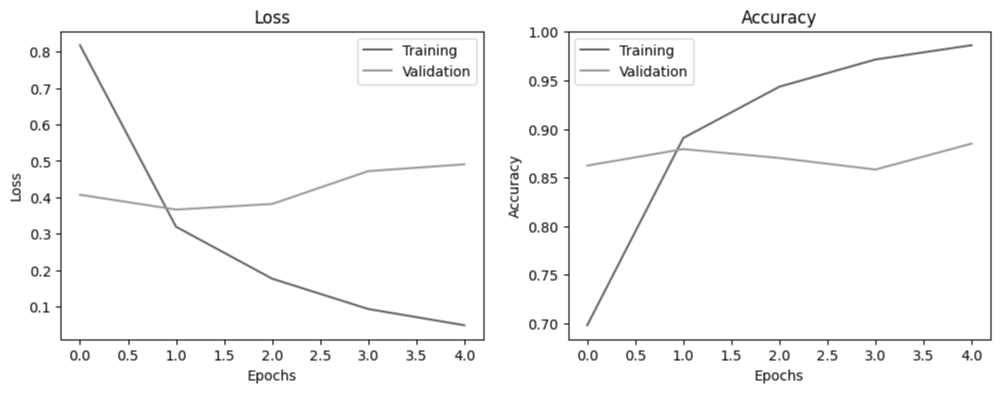
\includegraphics[width=0.85\textwidth]{Images/T LOSS EPOCH.png}  
    \caption{Transformer Epoch, Loss, Accuracy}
    \label{lstm t epch}  % Label for referencing the figure
\end{figure}


\pagebreak

\vspace*{-1cm}

\begin{figure}[h!]  
    \centering
    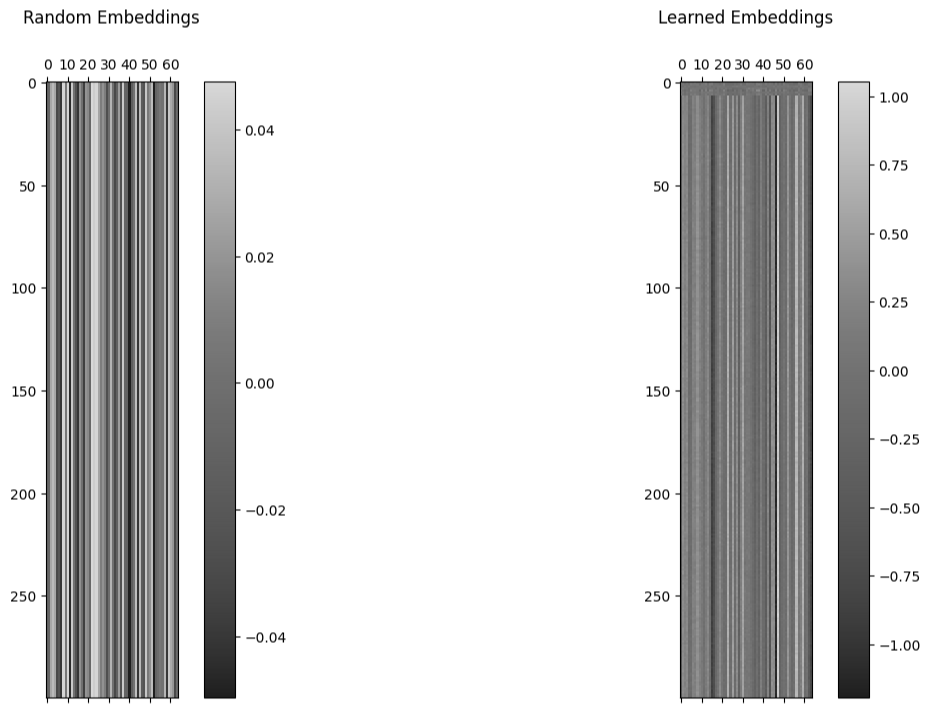
\includegraphics[width=0.7\textwidth]{Images/T EMBED.png}  
    \caption{Transformer Model Random and Learned Embeddings}
    \label{lstm t embed}  % Label for referencing the figure
\end{figure}

\vspace{-1cm}

% --------- ENSEMBLE LEARNING 1----------
\subsection{Ensemble Model}

\vspace{-0.5cm}

\begin{table}[H]
    \caption*{\textbf{General Stepwise Algorithm for Ensemble Models}}
    \label{tab:ensemble_algorithm}
    \centering
    \renewcommand{\arraystretch}{1.3}
    \small
    \setlength{\arrayrulewidth}{1pt}
    \begin{tabularx}{\textwidth}{|c|X|}
        \hlineB{1.0}
        \rowcolor{lightestgray}
        \textbf{Step} & \textbf{Description} \\
        \hlineB{1.0}
        1 & \textbf{Import Libraries:} Import required packages including \texttt{numpy}, \texttt{pandas}, \texttt{tensorflow} (Keras modules such as \texttt{MultiHeadAttention}, \texttt{Embedding}, etc.), \texttt{scikit-learn} (e.g., \texttt{RandomForestClassifier}, \texttt{train\_test\_split}, \texttt{confusion\_matrix}), and \texttt{pickle}. \\
        \hlineB{1.0}
        2 & \textbf{Load Pre-trained Base Models \& Vectorizers:} Load saved models and vectorizers using \texttt{pickle} and \texttt{load\_model}. Base models include: Logistic Regression (LR), Support Vector Machine (SVM), Naive Bayes (NB), XGBoost, LSTM, and Transformer. Also load corresponding vectorizers/tokenizers (e.g., \texttt{LRvectorizer}, \texttt{SVMvectorizer}, \texttt{NBvectorizer}, \texttt{tfidf\_vectorizer}, \texttt{LSTM\_tokenizer}, \texttt{Tvectorize\_layer}) and label encoders. \\
        \hlineB{1.0}
        3 & \textbf{Load \& Preprocess Test Data:} Read \texttt{preprocessed\_mental\_health.csv} with pandas, drop rows with missing \texttt{cleaned\_text}, extract texts and labels, and encode labels using \texttt{LabelEncoder}. \\
        \hlineB{1.0}
        4 & \textbf{Text Preprocessing for Each Model:} Transform the raw texts using respective vectorizers/tokenizers:
              \begin{itemize}[noitemsep, topsep=0pt]
                  \item LR, SVM, NB: Use \texttt{LRvectorizer}, \texttt{SVMvectorizer}, \texttt{NBvectorizer}.
                  \item XGBoost: Use \texttt{tfidf\_vectorizer}.
                  \item LSTM: Convert texts using \texttt{LSTM\_tokenizer} and apply \texttt{pad\_sequences}.
                  \item Transformer: Process texts using \texttt{Tvectorize\_layer}.
              \end{itemize} \\
        \hlineB{1.0}
        5 & \textbf{Generate Base Model Predictions:} For each base model, compute prediction probabilities:
              \begin{itemize}[noitemsep, topsep=0pt]
                  \item LR: \texttt{lr\_model.predict\_proba}
                  \item SVM: \texttt{svm\_model.predict\_proba}
                  \item NB: \texttt{nb\_model.predict\_proba}
                  \item XGBoost: \texttt{xgb\_model.predict\_proba}
                  \item LSTM: \texttt{lstm\_model.predict}
                  \item Transformer: \texttt{transformer\_model.predict}
              \end{itemize} \\
        \hlineB{1.0}
    \end{tabularx}
\end{table}

\begin{table}[H]
    \caption*{\textbf{General Stepwise Algorithm for Ensemble Models}}
    \label{tab:ensemble_algorithm}
    \centering
    \renewcommand{\arraystretch}{1.3}
    \small
    \setlength{\arrayrulewidth}{1pt}
    \begin{tabularx}{\textwidth}{|c|X|}
        \hlineB{1.0}
        \rowcolor{lightestgray}
        \textbf{Step} & \textbf{Description} \\
        \hlineB{1.0}
        6 & \textbf{Stack Predictions:} Horizontally stack all base model prediction probabilities to form a new feature matrix (\texttt{stacked\_features}) for the meta-learner. \\
        \hlineB{1.0}
        7 & \textbf{Ensemble Configuration \& Data Splitting:} Split the stacked features and true labels (using \texttt{train\_test\_split}) into training and testing sets. Specify ensemble configurations:
              \begin{itemize}[noitemsep, topsep=0pt]
                  \item \textbf{Ensemble Model 1:} Base models: LR, XGBoost; Meta-learner: XGBoost.
                  \item \textbf{Ensemble Model 2:} Base models: LR, NB, SVM, XGBoost, LSTM; Meta-learner: XGBoost.
                  \item \textbf{Ensemble Model 3:} Base models: LR, NB, SVM, XGBoost, LSTM; Meta-learner: Random Forest.
                  \item \textbf{Ensemble Model 4:} Same base models as in Ensemble Model 7 using Bagging.
                  \item \textbf{Ensemble Model 5:} Same base models as in Ensemble Model 7 using Blending.
                  \item \textbf{Ensemble Model 6:} Same base models as in Ensemble Model 7 using Weighted Voting.
                  \item \textbf{Ensemble Model 7:} Base models: LR, SVM, NB, LSTM, XGBoost, Transformer; Meta-learner: Random Forest.
              \end{itemize} \\
        \hlineB{1.0}
        8 & \textbf{Train Meta-Learner:} Train the meta-learner (e.g., Random Forest, XGBoost, or ensemble strategies like Bagging, Blending, Voting) on the training portion of the stacked feature matrix. \\
        \hlineB{1.0}
        9 & \textbf{Evaluate Ensemble Model:} Predict on the test set using the meta-learner and compute evaluation metrics: accuracy, classification report, and confusion matrix. Also, perform cross-validation (e.g., using \texttt{cross\_val\_score}) to assess stability. \\
        \hlineB{1.0}
        10 & \textbf{Output Results:} Print final evaluation metrics (accuracy, report, confusion matrix) and cross-validation results. \\
        \hlineB{1.0}
    \end{tabularx}
\end{table}


\subsection{Wellbeing Survey and Association Matrix}

\begin{figure}[H]  
    \centering
    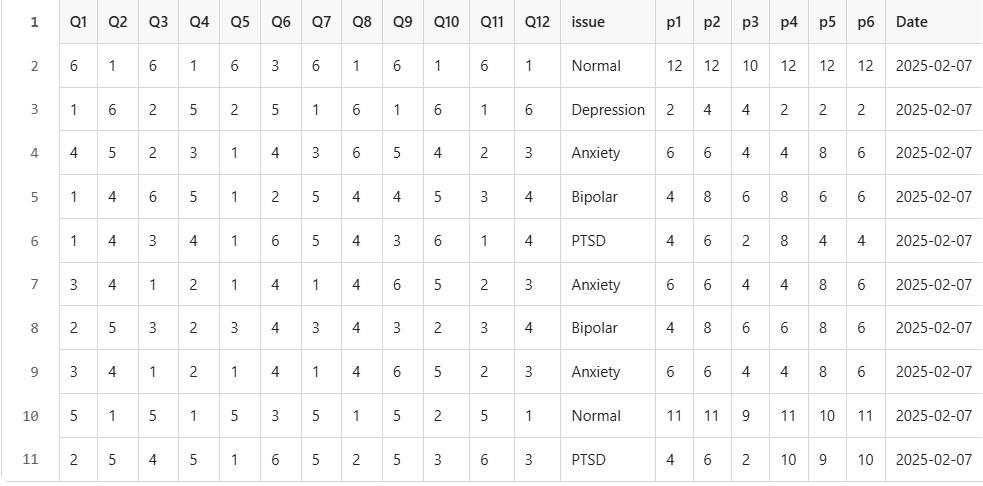
\includegraphics[width=0.8\textwidth]{App Images/32 Interface.png}  
    \caption{Sample Response Collection Sheet}
    \label{01i}  % Label for referencing the figure
\end{figure}

\pagebreak

\vspace*{-1.5cm}

\begin{table}[H]
    \caption*{Step-by-Step Algorithm for the Well-being Survey Option}
    \vspace{-0.5em}
    \label{tab:algorithm}
    \setlength{\arrayrulewidth}{1pt}
    \begin{tabularx}{\textwidth}{|l|X|X|}
    \hlineB{1.0}
    \rowcolor{lightestgray}
    \textbf{Step} & \textbf{Operation} & \textbf{Description / Formula} \\ \hlineB{1.0}
    1 & \textbf{Initialization:} \newline
    - Define file paths: \texttt{csv\_file\_path}, \texttt{image\_path}, \texttt{am\_file\_path}. \newline
    - Display title \textit{``Well-being Survey''}. & -- \\ \hlineB{1.0}
    2 & \textbf{Display Introductory Image:} \newline
    - Check if the image file exists at \texttt{image\_path} and display it. & --\\ \hlineB{1.0}
    3 & \textbf{Display Instructions:} \newline
    - Present informational messages and detailed instructions. \newline
    - Describe the Ryff Scale & 
    \[
    \begin{array}{l}
    \textbf{1} \quad \rightarrow \quad \text{Strongly Disagree} \\
    \textbf{2} \quad \rightarrow \quad \text{Disagree} \\
    \textbf{3} \quad \rightarrow \quad \text{Slightly Disagree} \\
    \textbf{4} \quad \rightarrow \quad \text{Slightly Agree} \\
    \textbf{5} \quad \rightarrow \quad \text{Agree} \\
    \textbf{6} \quad \rightarrow \quad \text{Strongly Agree}
    \end{array}
    \]
    \\ \hlineB{1.0}
    4 & \textbf{Load or Create Response Data:} \newline
    - Attempt to load \texttt{response.csv} into a DataFrame. \newline
    - If not found, create a new DataFrame with columns: \{Q1, Q2, \dots, Q12, issue, p1, \dots, p6, Date\}. \newline 
    - (R) against questions \{Q2, Q4, Q6, Q8, Q10, Q12\} signify reverse scoring & 
    \[
    \begin{array}{l}
    \textbf{Q1-Q2} : \text{Self Acceptance} \\
    \textbf{Q3-Q4} : \text{Positive relations with others} \\
    \textbf{Q5-Q6} : \text{Autonomy} \\
    \textbf{Q7-Q8} : \text{Environmental Mastery} \\
    \textbf{Q9-Q10} : \text{Purpose In Life} \\
    \textbf{Q11-Q12} : \text{Personal Growth}
    \end{array}
    \]
    \\ \hlineB{1.0}
    5 & \textbf{Collect User Responses:} \newline
    - Initialize an empty dictionary \texttt{responses}. \newline
    - \textbf{Q00:} Record predicted mental issue (via radio buttons with options: Anxiety, Bipolar, Depression, Normal, PTSD). \newline
    - \textbf{Q01--Q12:} Present 12 survey questions; record responses (scale 1--6). & \textbf{Follow these links for details:} \quad \newline \newline
    https://positivepsychology.com/ryff-scale-psychological-wellbeing/ \quad \newline \newline
    https://centerofinquiry.org/uncategorized\newline /ryff-scales-of-psychological-well-being/ \\ \hlineB{1.0}
    6 & \textbf{Append Current Date:} \newline
    - Add the current date in \texttt{YYYY-MM-DD} format to \texttt{responses}. & \(\text{Date} = \text{current date (YYYY-MM-DD)}\) \\ \hlineB{1.0}
    7 & \textbf{Overall Score Calculation:} \newline
    For each well-being parameter, compute a score using two survey responses. \newline
    \textbf{Variables:} \newline
    \(S_{\mathrm{SA}}\): Self Acceptance \newline
    \(S_{\mathrm{PR}}\): Positive Relations with Others  \newline
    \(S_{\mathrm{A}}\): Autonomy
    & 
    \[
    \begin{array}{c}
    S_{\mathrm{SA}} = Q1 + \left|7 - Q2\right|, \\
    S_{\mathrm{PR}} = Q3 + \left|7 - Q4\right|, \\
    S_{\mathrm{A}}  = Q5 + \left|7 - Q6\right|, \\
    S_{\mathrm{EM}} = Q7 + \left|7 - Q8\right|, \\
    S_{\mathrm{PL}} = Q9 + \left|7 - Q10\right|, \\
    S_{\mathrm{PG}} = Q11 + \left|7 - Q12\right|
    \end{array}
    \]
    \\ \hlineB{1.0}
    \end{tabularx}
\end{table}

\pagebreak

\vspace*{-1.5cm}

\begin{table}[H]
    \caption*{Step-by-Step Algorithm for the Well-being Survey Option}
    \label{tab:algorithm}
    \setlength{\arrayrulewidth}{1pt}
    \begin{tabularx}{\textwidth}{|l|X|X|}
    \hlineB{1.0}
    \rowcolor{lightestgray}
    \textbf{Step} & \textbf{Operation} & \textbf{Description / Formula} \\ \hlineB{1.0}
     & \(S_{\mathrm{EM}}\): Environmental Mastery \newline 
     \(S_{\mathrm{PL}}\): Purpose in Life  \newline
    \(S_{\mathrm{PG}}\): Personal Growth  &  \\ \hlineB{1.0}
    8 & \textbf{Determine Score Levels:} \newline
    - Compute the score level by dividing each parameter score by 2 (using integer division). \newline
    - Classify as: \textbf{Low} if score level is in \{1,2\}, \textbf{Medium} if in \{3,4\}, and \textbf{High} otherwise. & 
    \[
    \text{Score Level} = \left\lfloor \frac{S}{2} \right\rfloor,
    \]
    \[
    \begin{cases}
    \text{Low} & \text{if } S \in \{1,2\}, \\
    \text{Medium} & \text{if } S \in \{3,4\}, \\
    \text{High} & \text{if } S \geq 5.
    \end{cases}
    \]
    \\ \hlineB{1.0}
    9 & \textbf{Update Association Matrix:} \newline
    - For each parameter (\(p1\) to \(p6\)) and for each unique issue type in the responses, extract the corresponding values. \newline
    - Divide these values by 2, compute their mean, round the result to obtain an integer, and update the association matrix. & 
    \[
    \begin{array}{rcl}
    \text{For a parameter: } v_i &=& \dfrac{\text{value}}{2}, \\
    \bar{v} &=& \dfrac{1}{n} \sum_{i=1}^{n} v_i, \\
    \text{Final Value} &=& \mathrm{round}(\bar{v})
    \end{array}
    \] \\ \hlineB{1.0}
    10 & \textbf{Submit Responses and Save Data:} \newline
    - On clicking the \texttt{Submit Responses} button, display a success message. \newline
    - Append the new response entry to the DataFrame and update \texttt{response.csv}. \newline
    - Display the last 5 responses and count today’s respondents. & -- \\ \hlineB{1.0}
    11 & \textbf{Display Updated Association Matrix:} \newline
    - Call the function to update \texttt{am.csv} based on the latest responses, and display it as a table. & -- \\ \hlineB{1.0}
    \end{tabularx}
\end{table}
\
\vspace{-1.0cm}

\begin{figure}[H]  
    \centering
    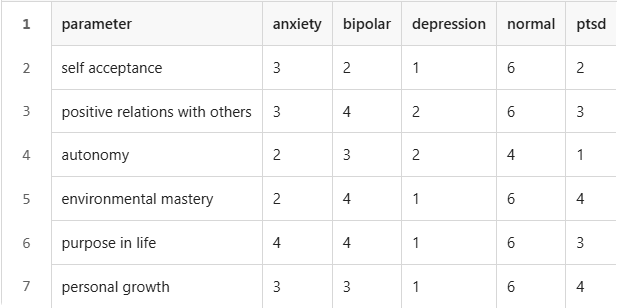
\includegraphics[width=0.7\textwidth]{App Images/33 Interface.png}  
    \caption{Sample Association Matrix}
    \label{01i}  % Label for referencing the figure
\end{figure}

\pagebreak

\begin{table}[H]
    \centering
    \caption*{Step-by-Step Algorithm for Association Matrix Analysis}
    \label{tab:algorithm}
    \setlength{\arrayrulewidth}{1pt}
    \begin{tabularx}{\textwidth}{|c|p{6cm}|>{\raggedright\arraybackslash}X|}
    \hlineB{1.0}
    \rowcolor{lightestgray}
    \textbf{Step} & \textbf{Operation} & \textbf{Mathematical Formula / Description} \\ \hlineB{1.0}
    1 & \textbf{Load Dataset} & Read the CSV file (e.g., \texttt{am.csv}) to obtain the association matrix data. \\ \hlineB{1.0}
    2 & \textbf{Define Row Names and Issue Columns} & Set row names: 
    \begin{tabular}[t]{@{}l@{}}self acceptance, positive relations with \\ others, autonomy, environmental mastery,\\ purpose in life, personal growth\end{tabular} \\ \hlineB{1.0}
    3 & \textbf{Extract Association Matrix} & \vspace{0.005em} Let \( \displaystyle A \in \mathbb{R}^{6 \times 5}, A_{ij} \text{ is the value for the }\) i\text{-th parameter} and j-th issue with issue columns ordered as: anxiety, bipolar, depression, normal, ptsd. \\ \hlineB{1.0}
    4 & \textbf{Define Probabilities Vector} & Define the probability vector where \(I_j\) refers to the mental issue probabilities. \newline
    \( \displaystyle \vec{p} = \begin{bmatrix} I1 \\ I2 \\ I3 \\ I4 \\ I5 \end{bmatrix}, \)
    which satisfies \( \displaystyle \sum_{j=1}^{5} I_j = 1 \).\newline \\ \hlineB{1.0}
    5 & \textbf{Weighted Sum Analysis} & Compute the weighted sum for each row: 
    \( \displaystyle w_i = \sum_{j=1}^{5} A_{ij}\, p_j, \quad i=1,\dots,6. \)
    Identify the row index with maximum \(w_i\), i.e., \( \displaystyle i^* = \arg\max_{i}\, w_i. \) \\ \hlineB{1.0}
    6 & \textbf{Cosine Similarity Analysis} & For each row vector \( \vec{a}_i \) of \(A\), compute:
    \( \displaystyle s_i = \frac{\vec{a}_i \cdot \vec{p}}{\|\vec{a}_i\|\,\|\vec{p}\|}, \quad i=1,\dots,6. \)
    Determine \( \displaystyle i^* = \arg\max_{i}\, s_i. \) \\ \hlineB{1.0}
    7 & \textbf{Euclidean Distance Analysis} & For each row, compute the Euclidean distance:
    \( \displaystyle d_i = \sqrt{\sum_{j=1}^{5} \left(A_{ij} - p_j\right)^2}, \quad i=1,\dots,6. \)
    Find the row index with the smallest distance:
    \( \displaystyle i^* = \arg\min_{i}\, d_i. \) \newline \\ \hlineB{1.0}
    8 & \textbf{Consensus Decision} & Compare the row names identified by the three analyses. If all three methods return the same row name, that is the consensus; otherwise, list the unique names obtained. \\ \hlineB{1.0}
\end{tabularx}
\end{table}

\begin{table}[H]
    \centering
    \caption*{Step-by-Step Algorithm for Association Matrix Analysis}
    \label{tab:algorithm}
    \setlength{\arrayrulewidth}{1pt}
    \begin{tabularx}{\textwidth}{|c|p{6cm}|>{\raggedright\arraybackslash}X|}
    \hlineB{1.0}
    \rowcolor{lightestgray}
    \textbf{Step} & \textbf{Operation} & \textbf{Mathematical Formula / Description} \\ \hlineB{1.0}
    9 & \textbf{Display Results} & Use Streamlit to display:
    \begin{itemize}[noitemsep, topsep=0pt]
        \item The original Association Matrix.
        \item The computed weighted sums, cosine similarity scores, and Euclidean distances.
        \item The row(s) corresponding to the maximum weighted sum, highest cosine similarity, and smallest Euclidean distance.
        \item The consensus result.
    \end{itemize} \\ \hlineB{1.0}
    \end{tabularx}
\end{table}

\subsection{RAG for Wellbeing Insights}

\begin{figure}[H]  
    \centering
    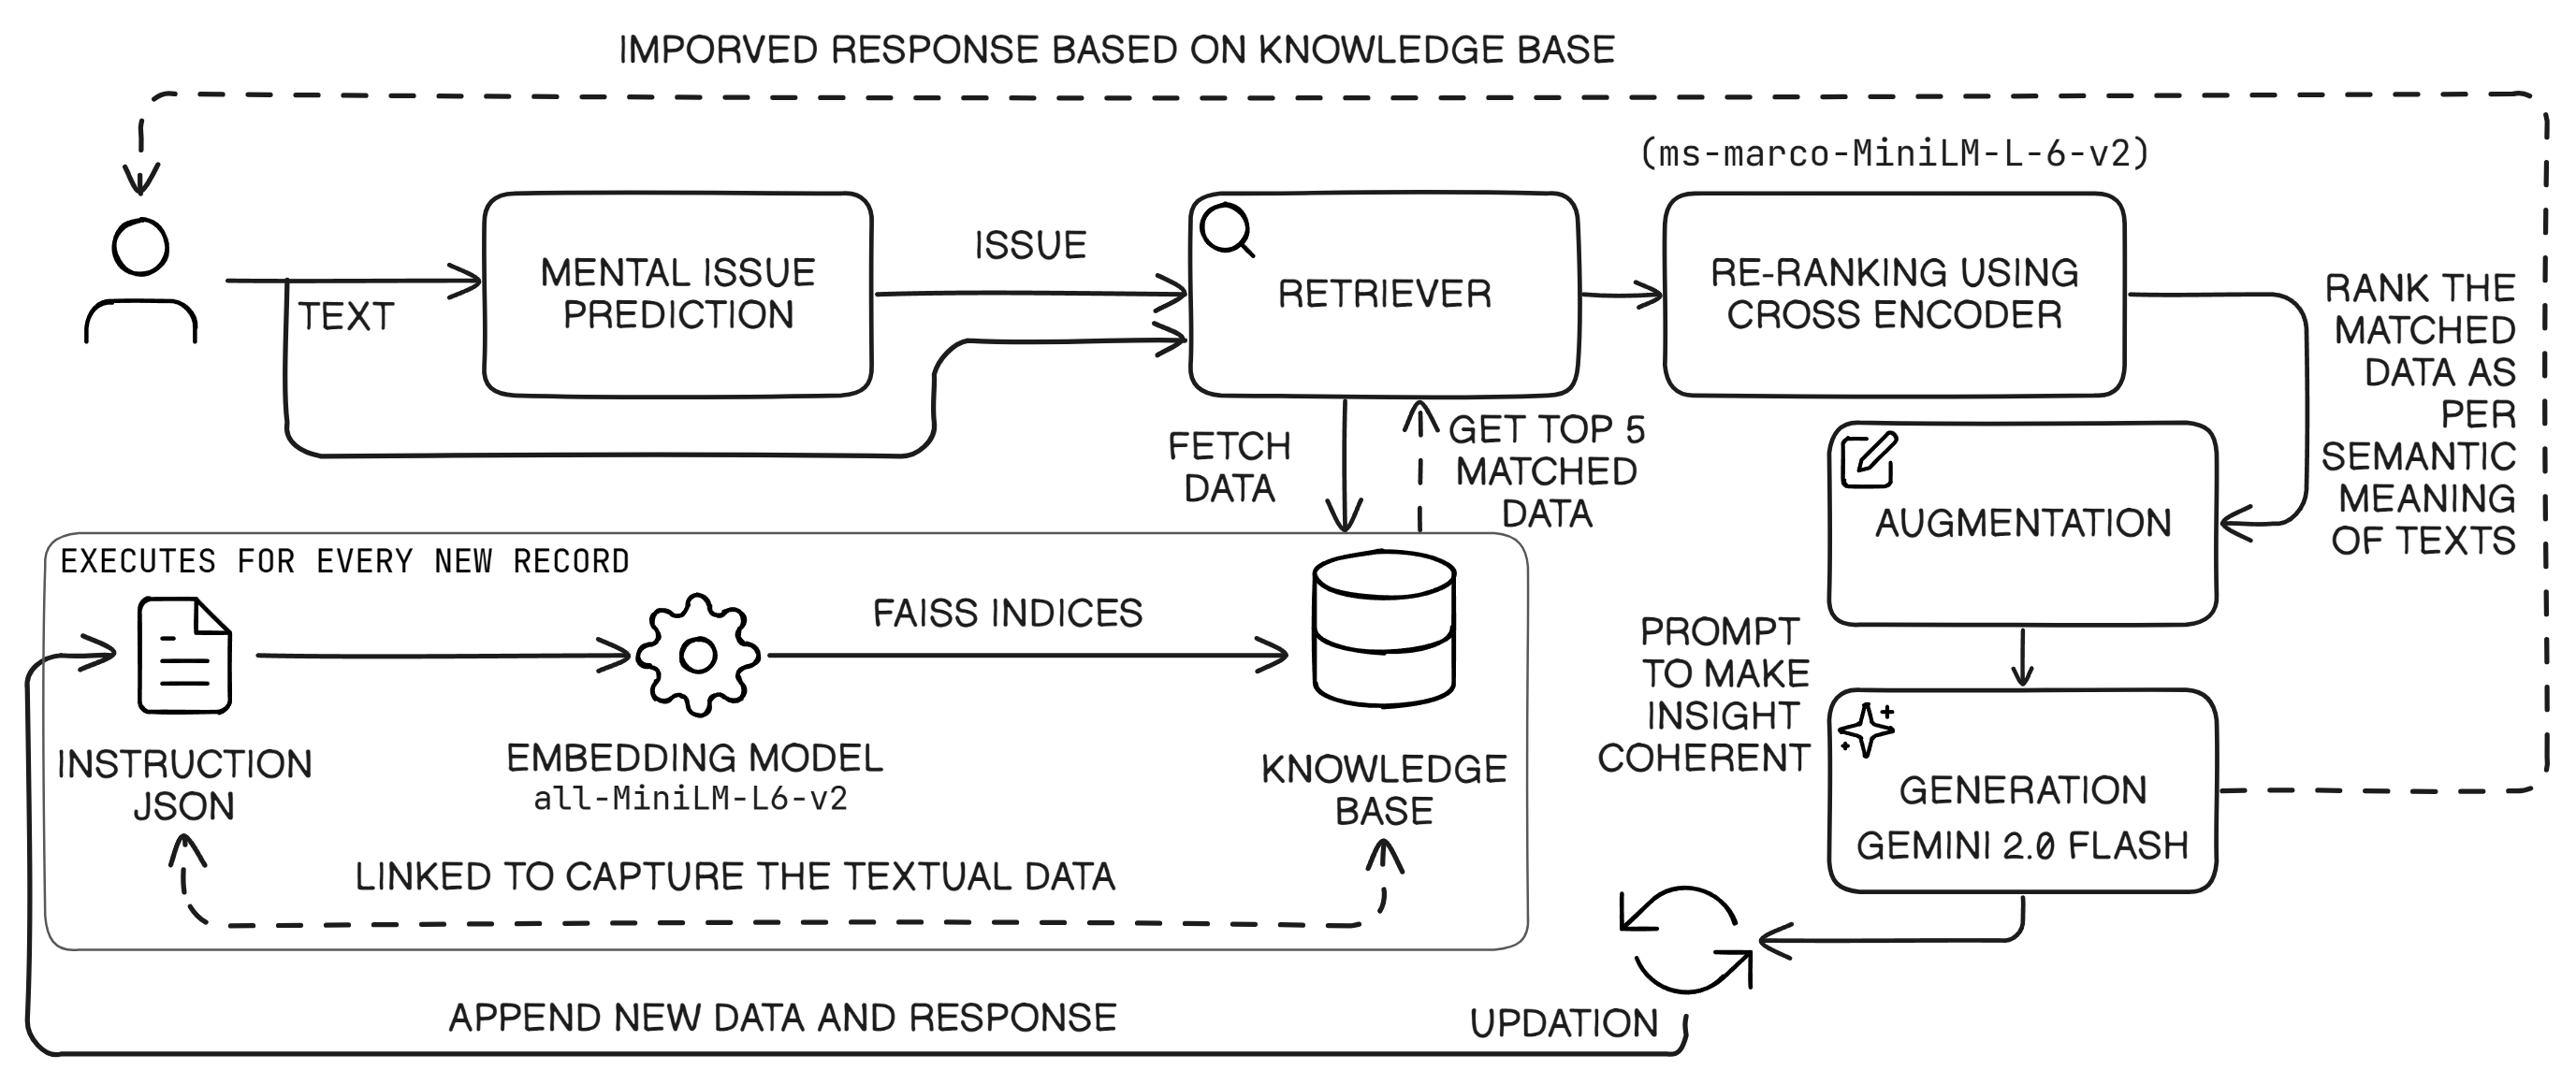
\includegraphics[width=0.8\textwidth]{Images/RAG_FLOW.png}  
    \caption{OVERVIEW OF RAG FOR GENERATING INSIGHTS}
    \label{01i}  % Label for referencing the figure
\end{figure}

\begin{table}[H]
    \centering
    \caption*{Step-by-Step Algorithm for RAG-based Wellbeing Insight Generation}
    \label{tab:algorithm}
    \setlength{\arrayrulewidth}{1pt}
    \begin{tabularx}{\textwidth}{|c|p{2.5cm}|X|}
        \hlineB{1.0}
        \rowcolor{lightestgray}
        \textbf{Step} & \textbf{Operation} & \textbf{Mathematical Formula / Description} \\ \hlineB{1.0}
        1 & \textbf{Import} \newline \textbf{Libraries} & Import necessary packages: \texttt{streamlit}, \texttt{json}, \texttt{pickle}, \texttt{numpy}, \texttt{faiss}, \texttt{sentence\_transformers}, \texttt{transformers}, \texttt{google.generativeai}, \texttt{plotly}, \texttt{sklearn.manifold.TSNE}, etc. \\ \hlineB{1.0}
        2 & \textbf{Configure Gemini API} & Set the generation configuration parameters and initialize the Gemini model. \\ \hlineB{1.0}
        3 & \textbf{Generate Instruction Dataset} & Create a dataset \texttt{instruction\_data.json} with \texttt{text}, \texttt{issue}, and \texttt{response} using Gemini API through batching and rate limiting. \\ \hlineB{1.0}
    \end{tabularx}
\end{table}

\pagebreak

\begin{table}[H]
    \centering
    \caption*{Step-by-Step Algorithm for RAG-based Wellbeing Insight Generation}
    \label{tab:algorithm}
    \setlength{\arrayrulewidth}{1pt}
    \begin{tabularx}{\textwidth}{|c|p{2.5cm}|X|}
        \hlineB{1.0}
        \rowcolor{lightestgray}
        \textbf{Step} & \textbf{Operation} & \textbf{Mathematical Formula / Description} \\ \hlineB{1.0}
        
        4 & \textbf{Build FAISS Index} & Load the saved model via: \texttt{embedding\_model = pickle.load("rag\_embedding\_gpu.pkl")}. Then load the instruction data from \texttt{instruction\_data.json} to form \texttt{documents = \{instruction + input\}} and \texttt{outputs = \{output\}}. Next, encode the documents using \texttt{embeddings = np.array([embedding\_model.encode(doc)])} so that embeddings $\in \mathbb{R}^{n \times d}$. Build the FAISS L2-index by setting \texttt{index = faiss.IndexFlatL2(d)} and calling \texttt{index.add(embeddings)}. Finally, save the tuple \texttt{\{documents, outputs, index, embeddings\}} into \texttt{"global\_store\_gpu.pkl"}. \\ \hlineB{1.0}


        5 & \textbf{Load Global Store} & Retrieve data from \texttt{global\_store\_gpu.pkl} (documents, indices, outputs and embeddings).
        \\ \hlineB{1.0}
        
        6 & \textbf{Compute Query} \newline \textbf{Embedding} & Create the query by concatenating user text and mental issue. Encode it and and cast to a float32 NumPy array:
        \vspace{-1em}
        \[
        \mathbf{v}_q = \text{embedding\_model.encode}(\text{query})
        \]
        \vspace{-1.5em}
        \\ \hlineB{1.0}
        
        7 & \textbf{FAISS} \newline \textbf{Retrieval} \newline \textbf{(Top-\(k\))} & 
        \begin{minipage}[t]{\linewidth}
        \begin{spacing}{0.4}
        Retrieve the top \(k=10\) matches using FAISS. The distance metric is the squared Euclidean (L2) norm:
        \[
        d(\mathbf{v}_q, \mathbf{v}_i) = \|\mathbf{v}_q - \mathbf{v}_i\|^2
        \]
        The query is processed as:
        \[
        (D, I) = \text{index.search}(\mathbf{v}_q, 5)
        \]
        \end{spacing}
        \end{minipage} \\ \hlineB{1.0}
        
        8 & \textbf{Re-ranking} & 
        \begin{minipage}[t]{\linewidth}
        \begin{spacing}{0.3}
        Re-rank the top \(n=5\) from the initially retrieved \(k\) documents to improve relevance using \texttt{ms-marco-MiniLM-L-6-v2}. \newline
        \begin{enumerate}[leftmargin=*, label=(\roman*)]
            \item Extract text for each candidate:
            \[
            \text{retrieved\_docs\_text} = \{ \text{documents}[i] \mid i \in \text{indices} \}
            \]
            \item Form pairs by concatenating the query with each document:
            \[
            \text{cross\_inp} = \{ [\text{query},\; \text{doc\_text}] \}.
            \]
            \item Compute cross-encoder scores:
            \[
            \text{cross\_scores} = \text{cross\_encoder.predict}(\text{cross\_inp}).
            \]
            \item Sort candidates by score in descending order
        \end{enumerate}
        \end{spacing}
        \end{minipage} \\ \hlineB{1.0}

        9 & \textbf{Filter by Ryff Parameters} & Apply text filtering to the retrieved output of the top candidate. Check if it contains any selected Ryff parameters (e.g., Autonomy, Positive Relations, etc.). \\ \hlineB{1.0}

        10 & \textbf{Generate} \newline \textbf{Refined} \newline \textbf{Insight} & Construct a prompt for the Gemini model based on the retrieved text and selected parameters. Generate a refined insight:
        \vspace{-1em}
        \[
        \text{generated\_output} = \text{gemini\_model.generate\_content}(\text{prompt})
        \] 
        \vspace{-2em}
        \\ \hlineB{1.0}
    \end{tabularx}
\end{table}

\pagebreak

\begin{table}[H]
    \centering
    \caption*{Step-by-Step Algorithm for RAG-based Wellbeing Insight Generation}
    \label{tab:algorithm}
    \setlength{\arrayrulewidth}{1pt}
    \begin{tabularx}{\textwidth}{|c|p{2.5cm}|X|}
        \hlineB{1.0}
        \rowcolor{lightestgray}
        \textbf{Step} & \textbf{Operation} & \textbf{Mathematical Formula / Description} \\ \hlineB{1.0}
    
        11 & \textbf{3D t-SNE} \newline \textbf{Visualization} & Combine the query embedding with the document embeddings and reduce the dimensionality using t-SNE:
        \[
        \text{reduced} = \text{TSNE}(n\_components=3)(\text{combined\_embeddings})
        \]
        Separate the query and top-\(k\) points for visualization via Plotly. \\ \hlineB{1.0}
        
        12 & \textbf{Plot Graph} & Plot the 3D scatter plot with annotations for the query, top-\(k\) matches, and connecting dotted lines. \\ \hlineB{1.0}
        
        13 & \textbf{Append New Record} & Append a new record to \texttt{instruction\_data.json} and rebuild the FAISS index. In this step, the updated documents are as below and the FAISS index is rebuilt with the new embeddings :
        \vspace{-0.5cm}
        \[
        \text{documents} = \{ \texttt{instruction} + \texttt{input} \}
        \]
        \vspace{-0.5cm}
         \\ \hlineB{1.0}
    \end{tabularx}
\end{table}

%\vspace{-0.7cm}

\begin{figure}[H]
  \centering
  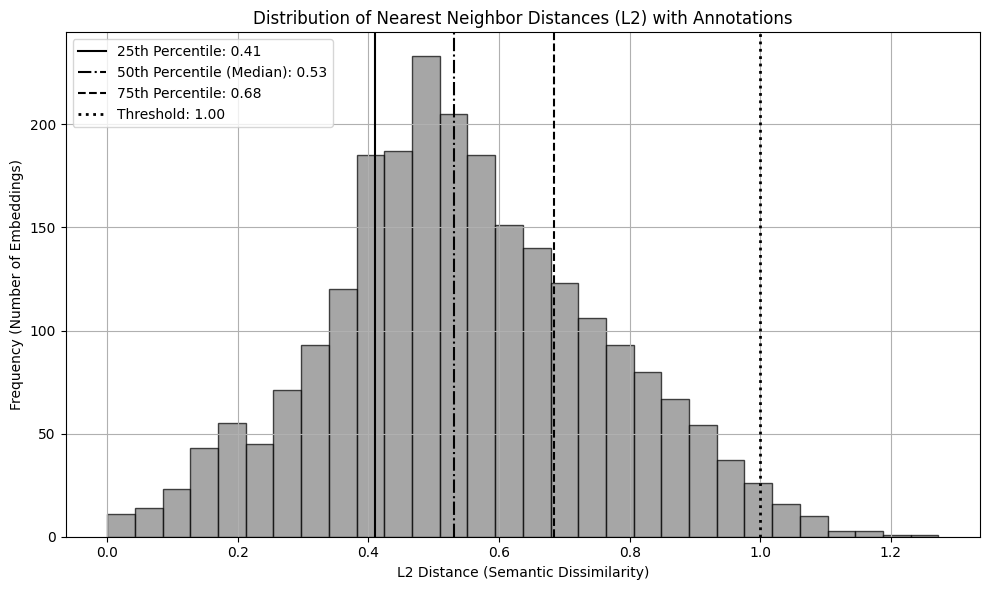
\includegraphics[width=1.0\textwidth]{Images/RAG_NEAR.png}
  \vspace{-0.35cm}
  \caption{Nearest Neighbours among the Embeddings}
  \label{fig:wellbeing_result}
\end{figure}

\pagebreak

\begin{figure}[H]
  \centering
  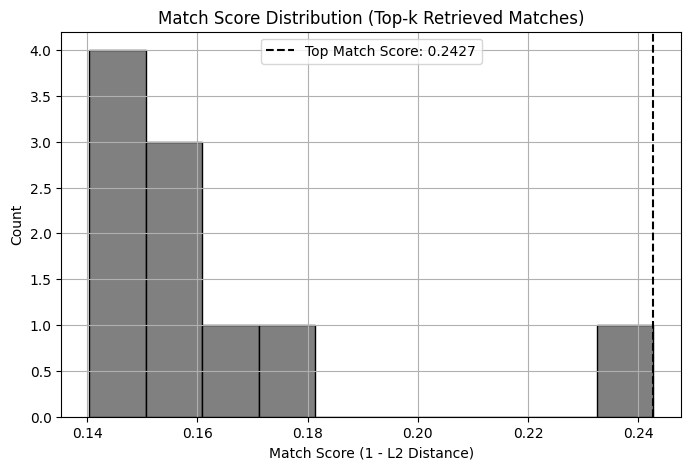
\includegraphics[width=1.0\textwidth]{Images/RAG_MATCHSCORE.png}
  \vspace{-0.75cm}
  \caption{Count of Matches and Top Score for an input}
  \label{fig:wellbeing_questions}
\end{figure}

\vspace{-0.625cm}

\begin{figure}[H]
    \centering
    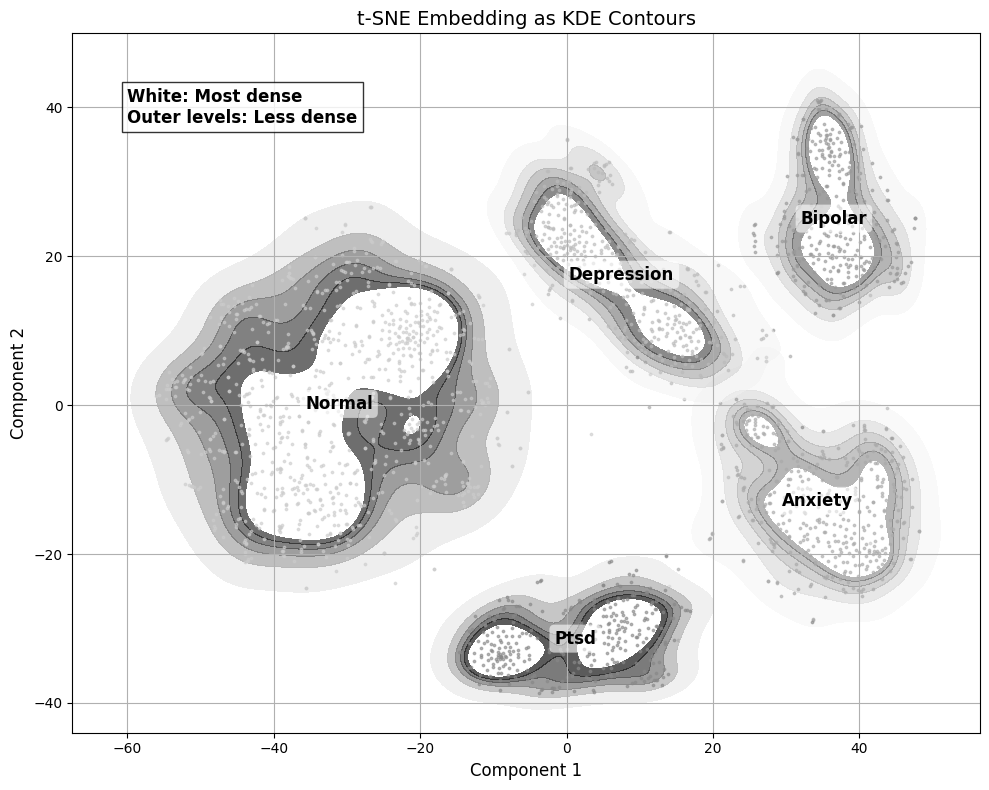
\includegraphics[width=1.0\textwidth]{Images/RAG_WBEMBED.png}
    \vspace{-0.75cm}
    \caption{Instruction Embeddings in 2D space}
    \label{fig:wellbeing_questions}
\end{figure}

\vspace{-2cm}

\pagebreak

\begin{figure}[H]
    \centering
    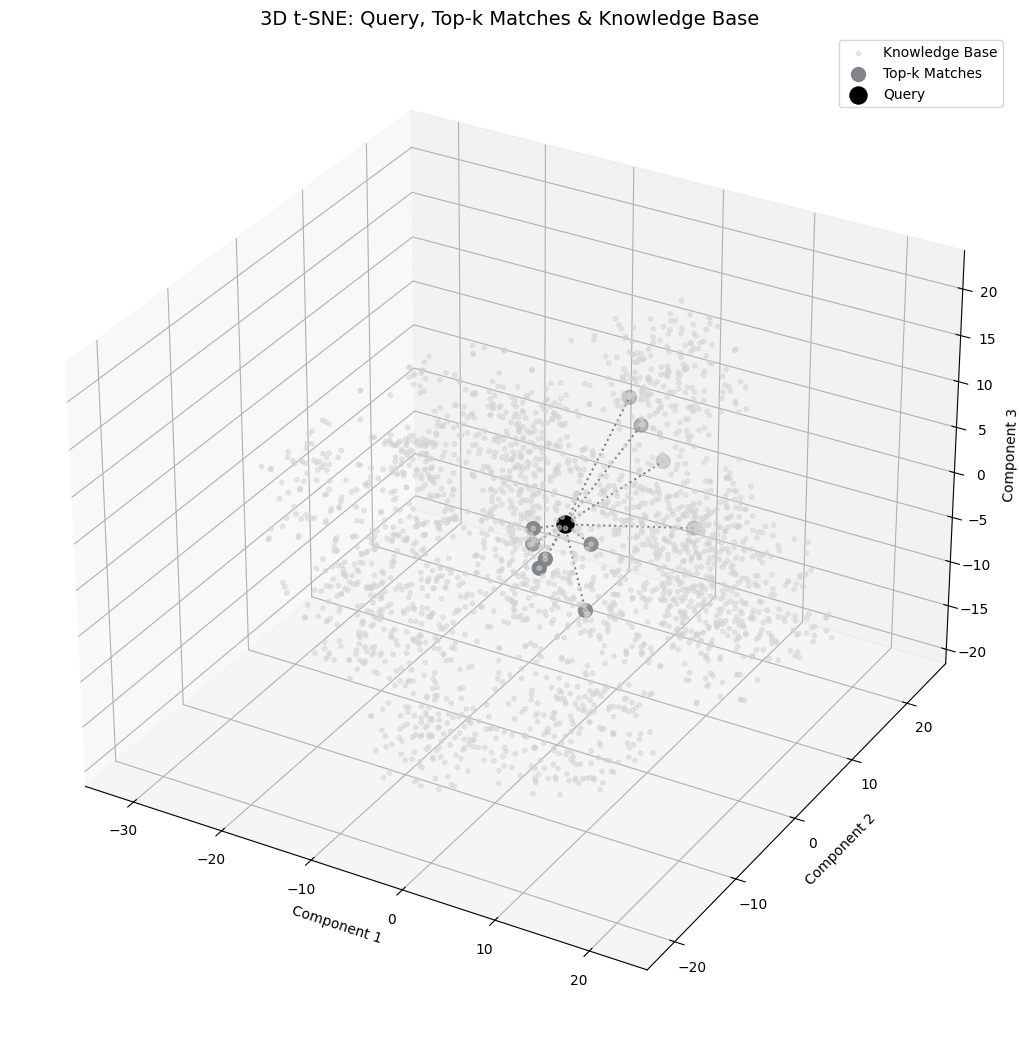
\includegraphics[width=0.8\textwidth]{Images/RAG_KNOWLEDGE.png}
    \vspace{-0.3cm}
    \caption{Visualization of Query and Top-\(k\) Matches}
    \label{fig:wellbeing_questions}
\end{figure}



% ------------------------- Implementation Ends -----------------------------
